\documentclass{beamer}
\mode<presentation>
\usetheme{CambridgeUS}
\usepackage[russian]{babel}
\usepackage[utf8]{inputenc}
\usepackage[T2A]{fontenc}
\usepackage{sansmathaccent}

\usepackage{verbatim}
\usepackage{alltt}

\pdfmapfile{+sansmathaccent.map}
\title[Logical]{Построение логической модели}
\author{Наумов Д.А., доц. каф. КТ}
\date[02.03.2020] {Базы данных и базы знаний, 2020}

\begin{document}

%ТИТУЛЬНЫЙ СЛАЙД
\begin{frame}
  \titlepage
\end{frame}
  
%СОДЕРЖАНИЕ ЛЕКЦИИ
\begin{frame}
  \frametitle{Содержание лекции}
  \tableofcontents  
\end{frame}
  
%РАЗДЕЛ 1
\section{Преобразование концептуальной модели в логическую}
\begin{frame}
\begin{center}
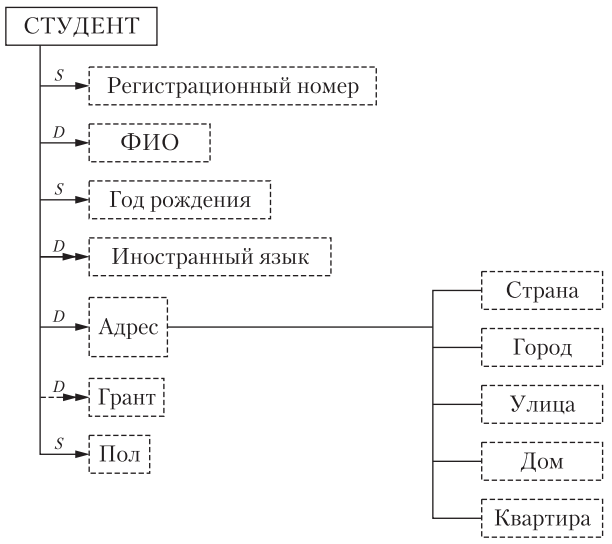
\includegraphics[scale=0.6]{images/lec03-pic02.png}
\end{center}
\end{frame}

\begin{frame}
\begin{center}
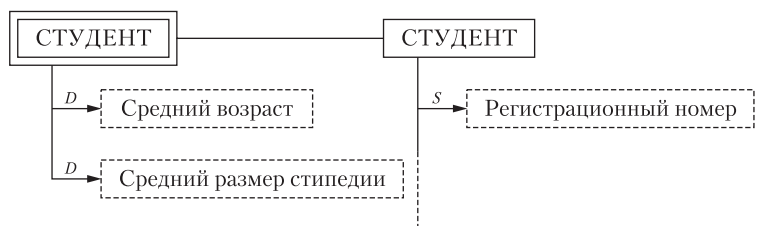
\includegraphics[scale=0.6]{images/lec03-pic03.png}
\end{center}
\end{frame}

\begin{frame}{Описание степени связей между сущностями}
\begin{center}

\includegraphics[scale=0.6]{images/lec03-pic04.png}
\end{center}
\end{frame}

\begin{frame}{Степень сязи 1:1}
\begin{center}
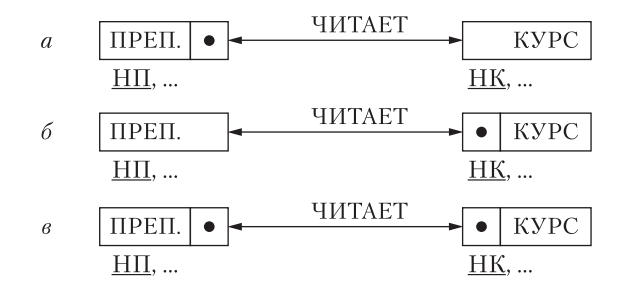
\includegraphics[scale=0.6]{images/lec03-pic05.png}
\end{center}
\end{frame}

\begin{frame}{Степень связи 1:M}
\begin{center}
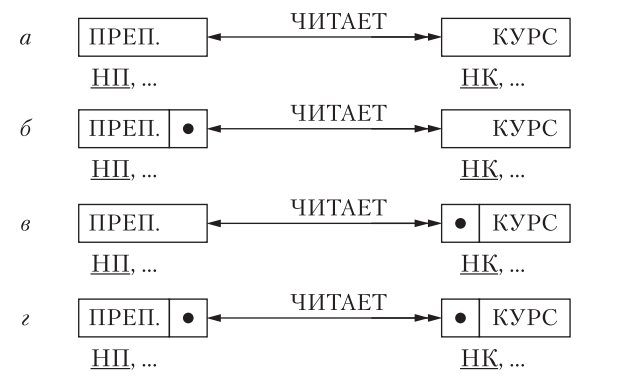
\includegraphics[scale=0.6]{images/lec03-pic06.png}
\end{center}
\end{frame}

\begin{frame}{Степень связи M:1}
\begin{center}
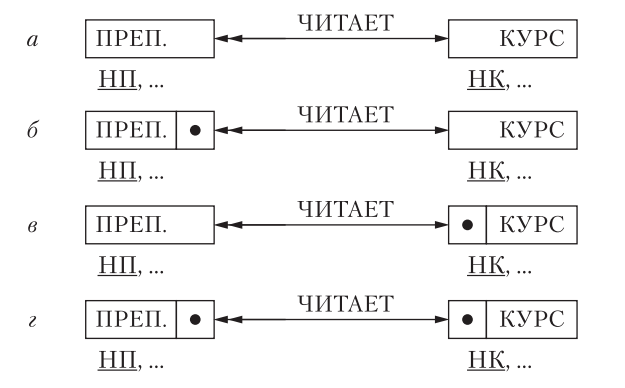
\includegraphics[scale=0.6]{images/lec03-pic07.png}
\end{center}
\end{frame}

\begin{frame}{Степень связи M:M}
\begin{center}
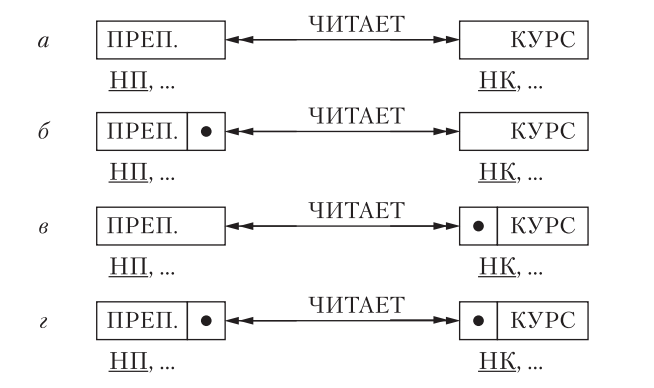
\includegraphics[scale=0.6]{images/lec03-pic08.png}
\end{center}
\end{frame}

\begin{frame}{Атрибуты-категории}
\begin{center}
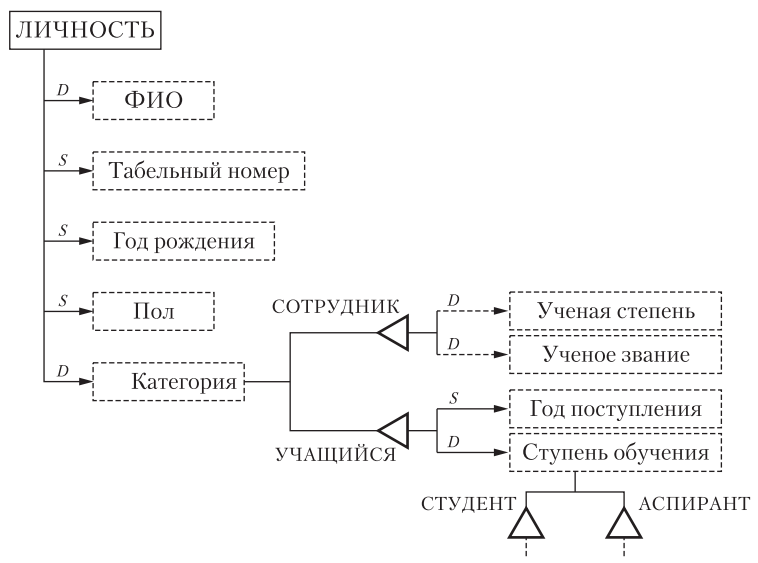
\includegraphics[scale=0.5]{images/lec03-pic09.png}
\end{center}
\end{frame}

\begin{frame}{Связь с атрибутами}
\begin{center}
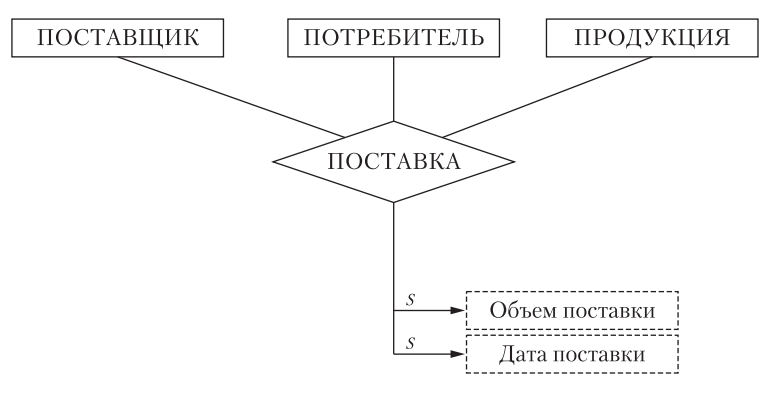
\includegraphics[scale=0.6]{images/lec03-pic10.png}
\end{center}
\end{frame}

\begin{frame}{Правило 1: Сущность и однозначаные атрибуты}
\begin{center}
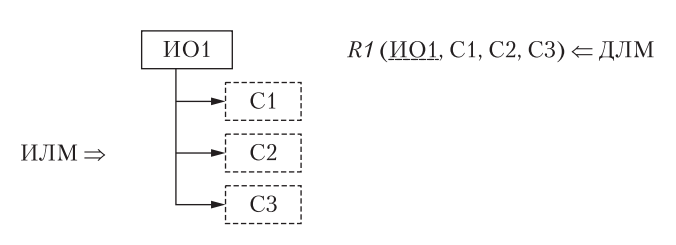
\includegraphics[scale=0.7]{images/lec03-pic11.png}
\end{center}
\end{frame}

\begin{frame}{Правило 2: Сущность и многозначаные атрибуты}
\begin{center}
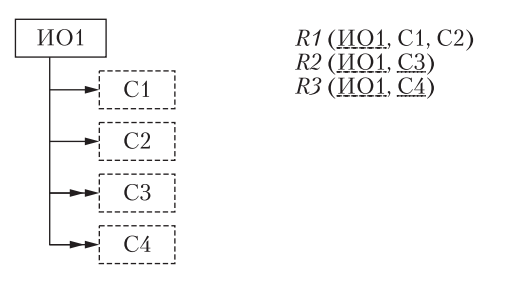
\includegraphics[scale=0.75]{images/lec03-pic12.png}
\end{center}
\end{frame}

\begin{frame}{Правило 3: Необязательный атрибут}
\begin{center}
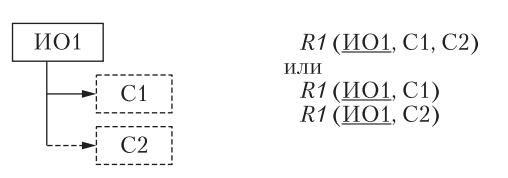
\includegraphics[scale=0.75]{images/lec03-pic13.png}
\end{center}
\end{frame}

\begin{frame}{Правило 4: Составной атрибут}
\begin{center}
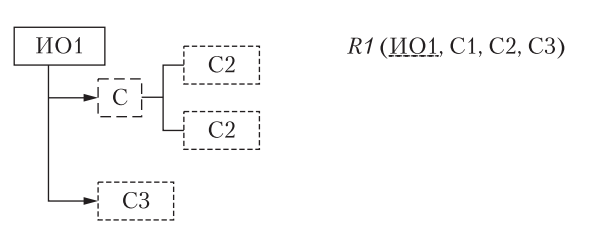
\includegraphics[scale=0.75]{images/lec03-pic14.png}
\end{center}
\end{frame}

\begin{frame}{Правило 5: Связь 1:1}
Вариант 1
\begin{center}
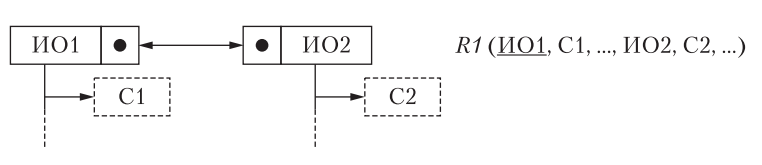
\includegraphics[scale=0.4]{images/lec03-pic15.png}
\end{center}
Вариант 2
\begin{center}
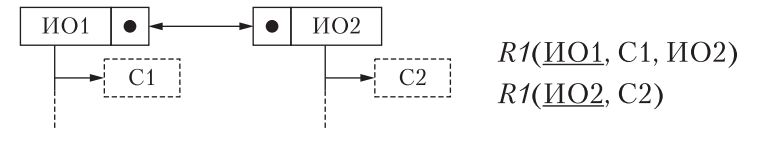
\includegraphics[scale=0.4]{images/lec03-pic16.png}
\end{center}
\end{frame}

\begin{frame}{Правило 5: Связь 1:1}
Вариант 3
\begin{center}
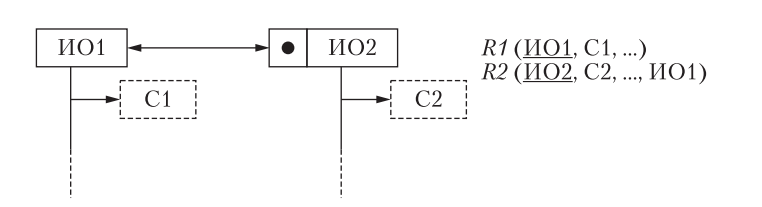
\includegraphics[scale=0.4]{images/lec03-pic17.png}
\end{center}
Вариант 4
\begin{center}
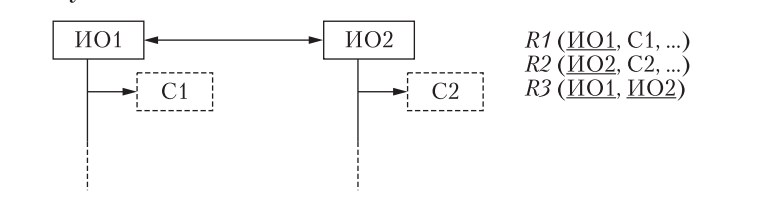
\includegraphics[scale=0.5]{images/lec03-pic18.png}
\end{center}
\end{frame}

\begin{frame}{Правило 6: Связь 1:M}
Вариант 1
\begin{center}
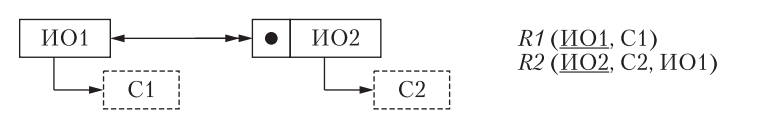
\includegraphics[scale=0.5]{images/lec03-pic19.png}
\end{center}
Вариант 2
\begin{center}
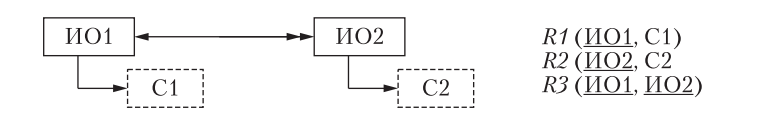
\includegraphics[scale=0.5]{images/lec03-pic20.png}
\end{center}
Вариант 3
\begin{center}
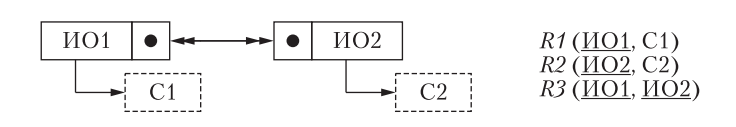
\includegraphics[scale=0.5]{images/lec03-pic21.png}
\end{center}
\end{frame}

\begin{frame}{Правило 7: Ассоциативная связь}
\begin{center}
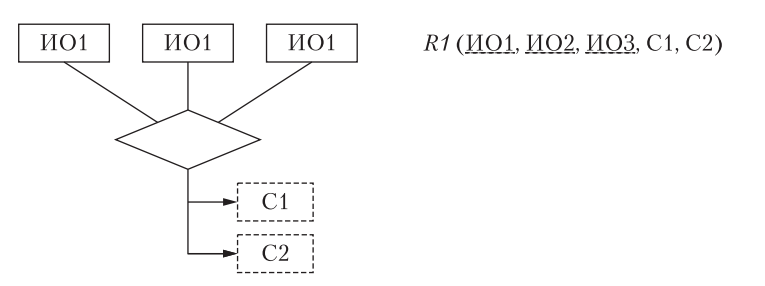
\includegraphics[scale=0.75]{images/lec03-pic22.png}
\end{center}
\end{frame}

\begin{frame}{Правило 8: Атрибуты-категории}
\begin{center}
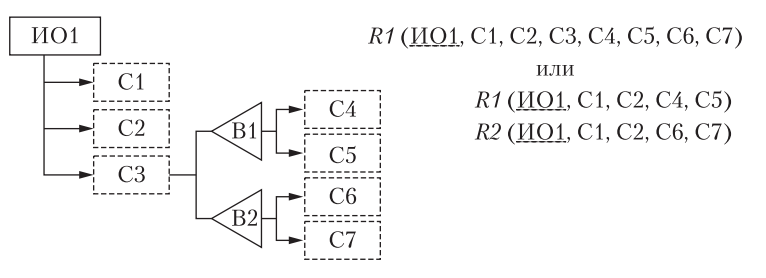
\includegraphics[scale=0.6]{images/lec03-pic23.png}
\end{center}
\end{frame}

\begin{frame}{Правило 9: Отношение обобщения}
\begin{center}
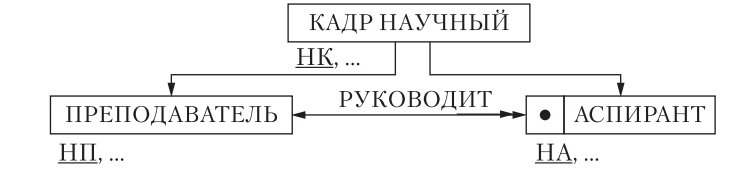
\includegraphics[scale=0.5]{images/lec03-pic24.png}
\end{center}
\begin{center}
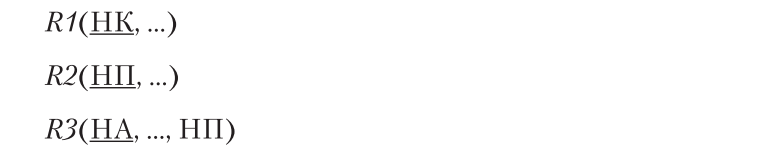
\includegraphics[scale=0.5]{images/lec03-pic25.png}
\end{center}
\end{frame}

\begin{frame}{Правило 10: n-арные связи}
\begin{center}
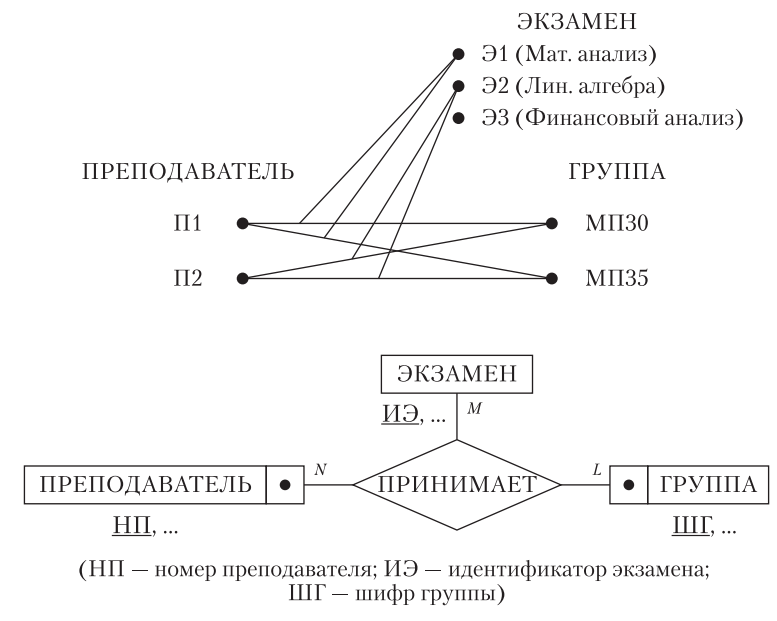
\includegraphics[scale=0.3]{images/lec03-pic26.png}
\end{center}
\begin{center}
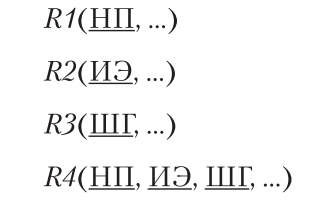
\includegraphics[scale=0.4]{images/lec03-pic27.png}
\end{center}
\end{frame}

\end{document}